\documentclass[11pt, letterpaper, twocolumn]{article}
\usepackage[english]{babel}
\usepackage{microtype}
\usepackage{amsmath,amsfonts,amsthm}
\usepackage[svgnames]{xcolor}
\usepackage{lastpage}
\usepackage{graphicx}
\usepackage{sectsty}
\allsectionsfont{\usefont{OT1}{phv}{b}{n}}
\usepackage{hanging}
\usepackage{xstring}
\usepackage{geometry}
\geometry{
	top=1cm,
	bottom=1.5cm,
	left=2cm,
	right=2cm,
	includehead,
	includefoot,
}
\setlength{\columnsep}{7mm}
\usepackage[T1]{fontenc}
\usepackage[utf8]{inputenc}
\usepackage{phfqit}
\usepackage{lettrine}
\usepackage{fix-cm}
\usepackage{XCharter}
\usepackage{fancyhdr}
\pagestyle{fancy}
\renewcommand{\headrulewidth}{0.0pt}
\renewcommand{\footrulewidth}{0.4pt}
\renewcommand{\sectionmark}[1]{\markboth{#1}{}}
\lhead{}
\chead{\textit{\thetitle}}
\rhead{}
\lfoot{}
\cfoot{}
\rfoot{\footnotesize Page \thepage\ of \pageref{LastPage}}
\fancypagestyle{firstpage}{ % Page style for the first page with the title
	\fancyhf{}
	\renewcommand{\footrulewidth}{0pt}
}
\newcommand{\authorstyle}[1]{{\large\usefont{OT1}{phv}{b}{n}\color{DarkRed}#1}}
\newcommand{\institution}[1]{{\footnotesize\usefont{OT1}{phv}{m}{sl}\color{Black}#1}}

\usepackage{titling}
\newcommand{\HorRule}{\color{DarkGoldenrod}\rule{\linewidth}{1pt}}
\pretitle{
	\vspace{-30pt} % Move the entire title section up
	\HorRule\vspace{10pt} % Horizontal rule before the title
	\fontsize{32}{36}\usefont{OT1}{phv}{b}{n}\selectfont % Helvetica
	\color{DarkRed} % Text colour for the title and author(s)
}

\posttitle{\par\vskip 15pt} % Whitespace under the title
\preauthor{}

\postauthor{
	\vspace{10pt}
	\par\HorRule
	\vspace{20pt}
}

\newcommand{\initial}[1]{
	\lettrine[lines=3,findent=4pt,nindent=0pt]{% Lettrine takes up 3 lines, the text to the right of it is indented 4pt and further indenting of lines 2+ is stopped
		\color{DarkGoldenrod}% Lettrine colour
		{#1}% The letter
	}{}}

\newcommand{\lettrineabstract}[1]{
	\StrLeft{#1}{1}[\firstletter]
	\initial{\firstletter}\textbf{\StrGobbleLeft{#1}{1}}}

\title{Entropy in DNA}

\author{
	\authorstyle{Lucas Blakeslee\textsuperscript{1}}
	\newline\newline
	\textsuperscript{1}\institution{Institute for Computing in Research. Santa Fe, New Mexico, United States of America}\\}

\date{\today}

%----------------------------------------------------------------------------------------

\begin{document}
	
	\maketitle % Print the title
	
	\thispagestyle{firstpage} % Apply the page style for the first page (no headers and footers)

	%	abstract

	\lettrineabstract{The entropy of a genomic sequence can provide a variety of insights into its nature, namely in that it can be an indicator of whether a region of DNA is expressed. This paper attempts to lay out the foundations for a new method of calculating entropy by bringing in information taken from the sequence's biological class. A normalized function was described that can identify the class of a sequence via subsequence comparison, which down the line can be used to create a definition for entropy specific to DNA.}

 
	\section{Background}
  Entropy as a measure of information content was described by Shannon (1948), whereupon he contributed immensely to founding the modern field of information theory. Where H is the entropy, and
  $p_{i}$ is the probability of a system being in state i (which can be thought
  of as the probability of i occurring), Shannon entropy is defined as:
  \begin{equation}
    	H(P)=-\sum _{i=1}p(i)\log p(i)
  \end{equation}
  Dividing the Shannon entropy by the information length can serve as normalization, resulting in what is called metric entropy \footnote{It is worth noting that there are multiple definitions of metric entropy, and the term often refers to entropy of a metric space}.

  An additional measure of entropy is topological entropy, originally designed as a descriptor of topological dynamical systems, but implemented for strings of finite length by Koslicki (2011). Koslicki's definition is as follows:
  
  \emph{If $w$ is a finite sequence of length $|w|$, and n is the unique integer such that:}
  $4^{n}+n-1 \leq |w| < 4^{n-1} +(n+1) -1$
  \begin{equation}
  	H_{top}(w) = \frac{\log_{4}(p_{w^{4^{n}+n -1}} (n))}{n}
  \end{equation}

  The most important conceptual difference between Shannon's and Koslicki's entropies is that the application of topological entropy ignores the frequency with which subsequences occur.
  
  The concept of entropy has been applied to a variety of physical systems, but what about
  biological ones? The question of entropy as it relates to biology was
  essentially first explored in Erwin Schrödinger's 1944 book \emph{What is
  Life?}, wherein he asked fundamental questions regarding how life requires
  \emph{negentropy} (in a later edition corrected by the author to free energy)
  in order to keep from decaying, and maintaining the decrease of entropy that evolution brings.

  Entropy as a measure of the complexity held within \emph{DNA} sequences has been described
  in the Shannonian sense by Schmitt \& Herzel (1997). The idea of block
  entropies is crucial for understanding the entropy of a DNA sequence. For a
  given alphabet $\aleph$ (here \{A, G, T, C\}), entropy will be low in
  a sequence $S$ when symbols and/or sub-sequences repeat. Classic Shannon
  entropy provides insight into the probabilities with which symbols occur,
  however, it does not provide insight into the relationships between different
  symbols. For that, \emph{block entropies} are required. The block entropy of a sequence can be defined as:

  \begin{equation}
    H_{n}= \sum _{i}p_{i}^{(n)}\log p_{i}^{(n)}
  \end{equation}

  Where $P_{i}^{(n)}$ are the probabilities of the combinations of $n$ symbols.
   
  The entropy of a DNA sequence can also bear insight into intron and exon regions (regions of DNA that aren't expressed and those that are), as intron regions aren't subject to the same evolutionary pressures to which exon regions are exposed, thus they would be expected to have a higher entropy (Koslicki, 2011).
  
  \section{Motivation}
   Here, I wondered whether a calculation of entropy for biological sequences could be defined given information about the class of the sequence. The idea here was that if knowledge was already had about common subsequences in a given sequence's class, an ``entropy reduction'' could be created to subtract from the raw entropy (which could be Shannonian or topological).
   
   \section{Methods}
   The first step in this process was being able to classify sequences into a biological class based on the subsequences (equivalent to blocks in block entropy) within the class of a genome. For proof of concept, two classes were used here: epsilonproteobacteria and gammaproteobacteria. For many members of each class, all subsequences up to length 15 within the bacterial genomes were counted, and the number of occurrences of each subsequence were averaged for each class.
   
   It was hypothesized that the Poisson distribution, a probability distribution that can estimate the number of occurrences of an event within a given period, could be used to predict the probabilities that an unknown sequence belongs to a given class based on the subsequences in the unknown sequences and the expected number of subsequences per class.
   
   The classic poisson distribution is:
   \begin{equation}
   	P(\lambda, k)={\frac {\lambda ^{k}e^{-\lambda }}{k!}}
   \end{equation}


   From which the following was derived:
   \begin{equation}
   	\ell(k_{i}, ^k\lambda_{i}) = \sum k_{i}\ln ^t\lambda_{i} + c
   \end{equation}
   where $\ell$ is the log probability.
   
   To put this into the terms of subsequences and classes:
   \begin{equation}
   	\ell(C_i, C_i\_expected\_T) = \sum C_i ln(C_i\_expected\_T)  + K\newline
   \end{equation}
   Where $C_i$ is the count of $i^{th}$ subsequence and $T$ is the type of organism. K is a constant unrelated to $C_i\_expected\_T$.
   
   The above was implemented, and the following plot was produced:
   \begin{center}
   	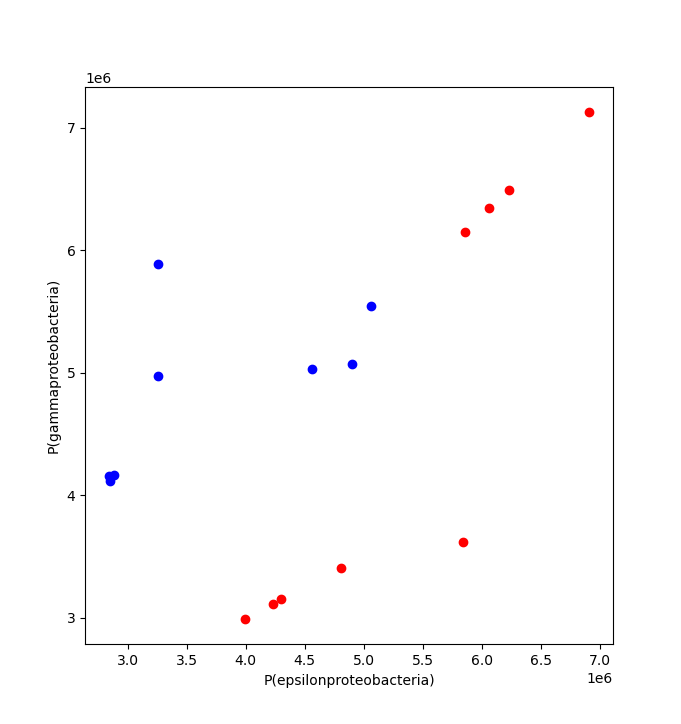
\includegraphics[scale=0.5]{find-likely-class-test.png}
   	\small{\textbf{Figure 1}}
   \end{center}

	Where blue dots are epsilonproteobacteria sequences, red dots are gammaproteobacteria sequences, and the (x, y) axes are the calculated probabilities for a sequence falling into the epsilonproteobacteria and gammaproteobacteria classes respectively.
	
	There is not clear separation, and the results of the function turned out not to be very meaningful for identifying species. One hypothesis as to why this might be has to do with microsatellites, which are blocks of DNA that repeat thousands to tens of thousands of times within a genome. Microsatellites are repeating sequences composed of small repeating blocks, such as $GCGCGCGC$, or $ATCATCATCATC$. Microsatellites may well not be Poisson random, and additionally do not seem to provide any special insight into what class a species falls into.
	
	With that in mind, the following function $f$ given the counts in an unknown sequence $C_{i}$, and the expected counts averaged from a class $E_{i}$ was defined:
	
	\begin{equation}
		f = \frac{\sum( \log(C_{i})  \log(E_{i}) )}{\sqrt{\sum(\log(C_{i})^{2})    \sum(\log(E_{i})^{2}))}}
	\end{equation}

	Where the denominator serves as a normalizing constant.
	
	\section{Results}
	The output of equation $7$ yielded much more clear separation between members of different classes than can be seen in Figure 1.
	
	\begin{center}
			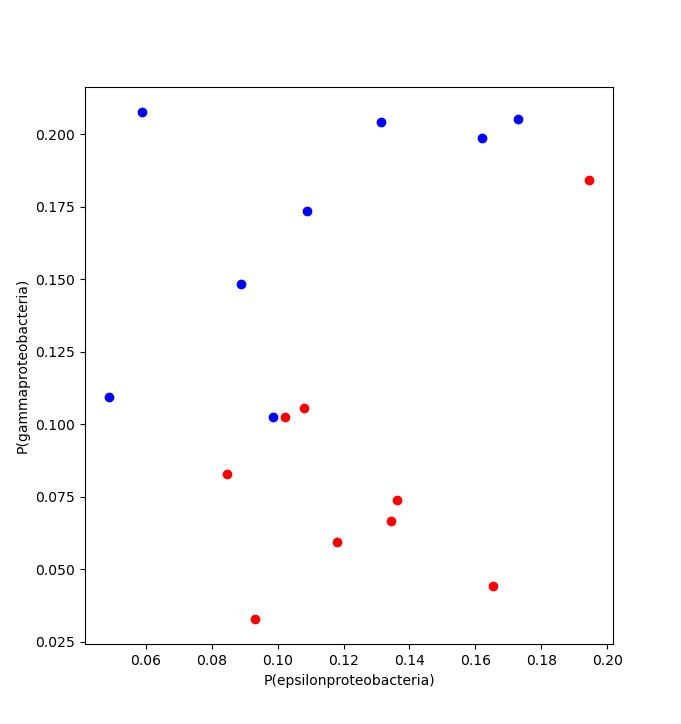
\includegraphics[scale=0.5]{func_test_2.png}
			\small{\textbf{Figure 2}}
	\end{center}

	A more-or-less diagonal separation can be seen between the gamma- and epsilonproteobacteria based on their calculated probabilities with a given class.
	
	Unfortunately, due to time constraints, the project had to be left here, but I plan to continue work on this project in a few areas.
	
	\subsection{Future Work}
	Going forward, crafting a definition for an entropy reduction to be subtracted from raw entropy is of prime importance. Performing these calculations on organisms of other classes (namely on eukaryotes and species with larger genomes and known intron regions) should yield further insight. Ultimately, I would like to map the genomes of organisms in an attempt to identify intron and exon regions, and see how the accuracy of intron/exon identification compares between that method, Shannon, and topological entropies.

	\section{Acknowledgments}
	I would sincerely like to thank my mentor, David Palmer of the Los Alamos National Laboratory, for the truly invaluable guidance and help he has provided me throughout this process.
	
	Additionally, I would like to thank the Institute for Computing in Research for providing me with the opportunity to perform this research.
	
	\section{References}
	\begin{hangparas}{.25in}{1}
		Koslicki, D. (2011). Topological entropy of DNA sequences. \emph{Bioinformatics}, 27(8), 1061–1067. https://doi.org/10.1093/bioinformatics/btr077 
		
		Schmitt, A. O., \& Herzel, H. (1997). Estimating the Entropy of DNA Sequences. \emph{Journal of Theoretical Biology}, 188(3), 369–377. https://doi.org/10.1006/jtbi.1997.0493 
		
		Schrödinger, E. (1944). What is Life? \emph{Cambridge University Press}
		
		Shannon, C. E., \& Weaver, W. (1949). The mathematical theory of communication. \emph{Urbana: University of Illinois Press}.
	\end{hangparas}
	
\end{document}
